\documentclass[aspectratio=169]{beamer}
\usetheme[block=fill]{metropolis}
\usepackage{tikz}
\usetikzlibrary{shapes.geometric, arrows.meta, positioning, calc}

\title{Building a Reproducible Scholarly Search Toolkit}
\subtitle{Episode 19: The E2E Integration Test}
\author{Scholar Search Kit}
\date{}

\begin{document}

\begin{frame}[plain]
  \titlepage
\end{frame}

\begin{frame}{Episode Goal}
  \begin{alertblock}{The Goal}
    Write a comprehensive End-to-End (E2E) test that executes the CLI, writes files to disk, and verifies the final output formats.
  \end{alertblock}
  \vspace{0.5cm}
  Unit tests verify that functions work. Integration tests verify that the system works when a user presses enter.
\end{frame}

\begin{frame}{The E2E Test Flow}
  \begin{center}
  \resizebox{0.8\linewidth}{!}{
  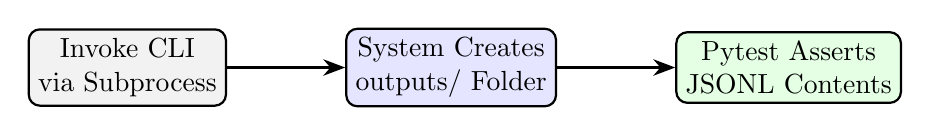
\begin{tikzpicture}[
      node distance=1cm and 1.5cm,
      cmd/.style={rectangle, draw, thick, rounded corners, minimum width=2.5cm, align=center, fill=black!5},
      sys/.style={rectangle, draw, thick, rounded corners, minimum width=2.5cm, align=center, fill=blue!10},
      verify/.style={rectangle, draw, thick, rounded corners, minimum width=2.5cm, align=center, fill=green!10},
      arrow/.style={-{Stealth[scale=1.2]}, thick}
    ]
    
    \node[cmd] (cli) {Invoke CLI\\via Subprocess};
    \node[sys, right=of cli] (file) {System Creates\\outputs/ Folder};
    \node[verify, right=of file] (chk) {Pytest Asserts\\JSONL Contents};
    
    \draw[arrow] (cli) -- (file);
    \draw[arrow] (file) -- (chk);
  \end{tikzpicture}
  }
  \end{center}
\end{frame}

\begin{frame}{Implementation: `tmp_path`}
  \begin{block}{Pytest Fixtures}
    Never let tests write to the real file system. They will leave garbage behind and fail randomly in parallel.
  \end{block}
  
  \begin{itemize}
      \item We use pytest's built-in \texttt{tmp\_path} fixture to create a temporary directory.
      \item We pass \texttt{--output-dir \{tmp\_path\}} to the CLI argument.
      \item Pytest deletes the directory automatically when the test finishes.
  \end{itemize}
\end{frame}

\begin{frame}{Implementation: Verifying JSONL}
  \begin{block}{Not Just File Existence}
    Checking if \texttt{results.jsonl} exists isn't enough. We must open it.
  \end{block}
  
  \begin{itemize}
      \item Read every line using \texttt{json.loads()}.
      \item Assert that the number of lines matches our \texttt{InMemoryProvider} mock count minus the duplicates stripped out.
  \end{itemize}
\end{frame}

\begin{frame}{Verification}
  \begin{alertblock}{Success Criteria}
    \begin{itemize}
        \item The test passes successfully without connecting to the internet.
        \item Running \texttt{pytest tests/} shows 100\% passing, proving our entire library is sound from start to finish.
    \end{itemize}
  \end{alertblock}
\end{frame}

\end{document}
